\chapter{Grafos}
\label{cap:grafos}

Grafos são estruturas discretas que consistem em vértices, e arestas que
conectam estes vértices. Existem vários tipos de grafos, dependendo da
existência de uma direcção nas arestas, de acordo a possibilidade de várias
arestas se interligarem ao mesmo par de vértices e de acordo a existência de
\emph{loops} ou repetições.
Problemas em quase todas as disciplinas podem resolvidos utilizando modelos de
grafos. Iremos apresentar alguns exemplos para ilustrar como os grafos são
utilizados como modelos numa variedade de aéras. Por exempo, iremos mostrar como
os grafos são utilizados para representar a competição de diferentes espécias
num nicho ecológico, e como os grafos são usados para representar quem
influencia quem numa organização e etc.

Utilizando modelos de grafos, podemos determinar se é possível caminhar todas as
ruas de uma cidade sem psasar por uma rua duas vezes, e podemos determinar o
número de cores necessário para colorar as regiões de um mapa. Grafos podem ser
utilizados para determinar se um circuito pode ser implementado numa placa de
circuitos plana. Podemos distinguir entre dois compostos químicos com a mesma
fórmula molecular mas estruturas diferentes utilizando grafos. Podemos
determinar se dois computadores estão conectados por um \emph{link} de
comunicação utilizando modelos gráficos de redes. Grafos com pesos atribuidos as
suas arestas podem ser utilizados para resolver problemas como encontrar o
caminho mais curto entre duas cidades numa rede de transporte. Neste capítulo
iremos apresentar os conceitos básicos da teoria dos grafos e apresentar alguns
modelos de grafos. Para resolver uma boa parte dos problemas que podem ser
estudados utilizando grafos, iremos apresentar alguns algoritmos de grafos.
Iremos também estudar a complexidade destes algoritmos.

\section{Grafos e Modelos de Grafos}

Começamos com a definição de grafos.
\begin{defn}
\label{def51}
Um \emph{grafo} $G = (V,E)$ consiste em $V$, um conjunto não-vazio de
\emph{vértices} (ou \emph{nós}) e $E$, um conjunto de \emph{arestas}. Cada
aresta possui ou um ou mais vértices associados a esta, chamada de sua
\emph{extremidade}. Diz-se que uma aresta \emph{conecta} as suas extremidades.
\end{defn}

\begin{description}
\item[\emph{Nota}:] O conjunto de vértices $V$ de um grafo $G$ pode ser
infinito. Um grago com um conjuntos infinito de vértices ou um
número infinito de arestas é chamado de \textbf{grafo infinito}, e em comparação, um grafo com
um conjunto de finito de vértices e um conjunto finito de arestas é chamado de
\textbf{grafo finito}. Neste manual iremos considerar apenas grafos finitos.
\end{description}

Agora imagine que uma rede de computadores é formada por centros de dados e
\textit{links} de comunicação entre computadores. Podemos representar a
localização de cada centro de dados por um ponto e cada \textit{link} de
comunicação por um segmento de linha, como mostra a Figura \ref{fig51}

\begin{figure}[H]
	\centering
	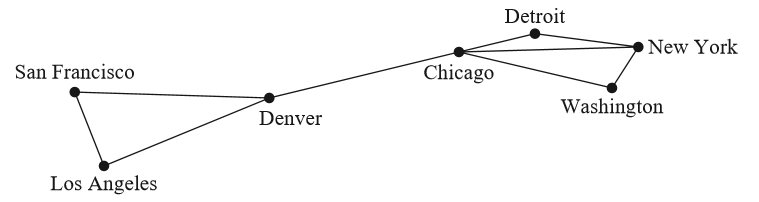
\includegraphics[scale=1]{chapter/imagens/51}
	\caption{Uma Rede de Computadores.}
	\label{fig51}
\end{figure}

Esta rede de computadores pode ser modelada utilzando grafos em que os vértices
do grafo representam centros de dados e as areas representam os \textit{links}
de comunicação. No geral, visualizamos os grafos usando pontos para represtentar
os vértices e segmentos de linha, possivelmente curvos, para representar as
arestas, onde as extremidades de um segmento de linha representando uma aresta
são os pontos representando as extremidades da aresta. Quando desenhamos um
grafo, geralmente tentamos desenhar as arestas de formas a não se cruzarem. No
entanto, isto não é necessário porque qualquer representação utilizando pontos
para representar os vértices e qualquer forma de conexão entre os vértices pode
ser utilizada. De facto, existem alguns grafos que não podem ser desenhados no
plano sem que as arestas se cruzem (veja a Secção \ref{sec:107}). O ponto
principal é que a forma como desenhamos um grafo é arbritária, desde que as
conexões correctas entre os vértices estejam representadas.

Note que cada aresta do grafo representando esta rede de computadores conecta
dois vértices diferentes. Isto é, nenhuma aresta conecta um vértice a si
próprio. Além disso, duas arestas diferentes não conectam o mesmo par de
vértices. Um grafo em que cada aresta conecta dois vértices diferentes e em que
duas arestas conectam o mesmo par de vértices é chamada de \textbf{grafo
simples}. Note que num grafo simples, cada aresta está associada à um par
não-ordenado de vértices, e mais nenhuma aresta está associada a esta mesma
aresta. Consequentemente, quando existe uma aresta de um grafo simples associada
a $\{u,v\}$, também podemos dizer, sem possibilidade de confusão, que $\{u,v\}$
é uma aresta do grafo.

Uma rede de computadores pode conter múltiplas ligações entre centros de dados,
como ilustrado na Figura \ref{fig52}. Para modelar tais redes precisamos de
grafos que posuam mais de uma aresta conectando o mesmo par de vértices. Grafos
que possam ter \textbf{múltiplas arestas} a conectar os mesmos vértices são
chamados de \textbf{multigrafos}. Quando existem $m$ arestas diferentes
associadas ao mesmo par não-ordenado de vértices $\{u,v\}$, também dizemos que
$\{u,v\}$ é uma aresta de multiplicidade $m$. Isto é, podemos pensar neste
conjunto de arestas como $m$ diferentes cópias de uma aresta $\{u,v\}$.

\begin{figure}[H]
	\centering
	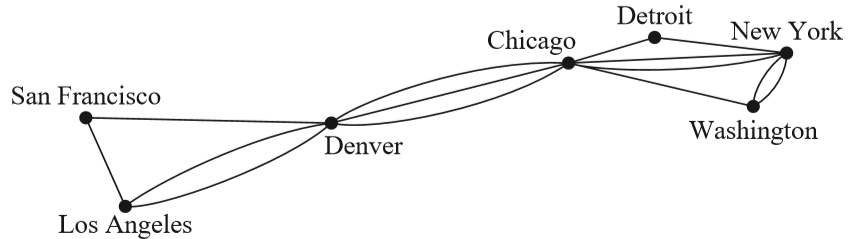
\includegraphics[scale=1]{chapter/imagens/52}
	\caption{Uma Rede de Computadores com Múltiplos LInks entre Centros de Dados.}
	\label{fig52}
\end{figure}

Por vezes um \textit{link} de comunicação de conecta um centro de dados consigo
próprio, possivelmente um laço de realimentação para diagnóstico. Uma rede deste
tipo é ilustrada na Figura \ref{fig53}. Para modelar esta rede precisamos
incluir arestas que conectem um vértice consigo próprio. Tais arestas são
chamadas de \textbf{laços} e as vezes podemos até ter mais de um laço no
vértice. Grafos que podem incluir laços, e possivelmente múltiplas arestas
conectando o mesmo par de vértices ou um vértice consigo próprio, são por vezes
chamados de \textbf{pseudo-grafos}.

\begin{figure}[H]
	\centering
	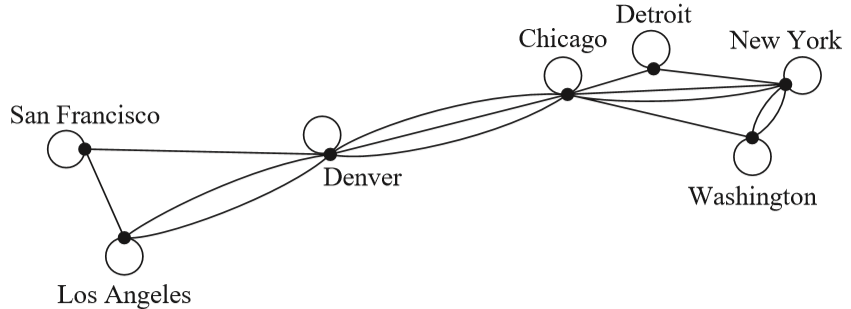
\includegraphics[scale=1]{chapter/imagens/53}
	\caption{Uma Rede de Computadores com Links para Diagnósticos.}
	\label{fig53}
\end{figure}


Até agora os grafos que apresentamos são \textbf{grafos não-direccionados}. As
suas arestas também são chamadas de \textbf{não direccionadas}. No entanto, para
construir um modelo de grafo, talvez achemos necessário atribuir direcções às
arestas do grafo. Por exemplo, numa rede de computadores, alguns \emph{links}
poderão operar apenas em uma direcção (tais ligaçõs são chamadas de linhas
\emph{duplex} simples). Isto pode ser o caso quando existe uma quantidade enorme
de tráfego enviada para alguns centros de dados, com pouco ou nenhum tráfego na
direcção oposta.

Para modelar tais redes de computadores utilizamos um grafo direccionado. Cada
aresta de um grafo direccionado está associada à um par ordenado. A definição de
um grafo direccionado que apresentamos aqui é mais geral do que a utilizada no
Capítulo \ref{cap:relacoes}, onde utilizamos grafos direccionados para
representar relações.

\begin{defn}
\label{def52}
Um \emph{grafo direccionado} (ou \emph{digrafo}) $(V,E)$ consiste num conjunto
não-vazio de vértices $V$ e um conjunto de \emph{arestas direccionadas} (ou
\emph{arcos}) $E$. Cada aresta direccionada está associada à um par ordenado de
vértices. A aresta direccionada associada ao par ordenado $(u,v)$ é dita que
\emph{começa} em $u$ e \emph{termina} em $v$.
\end{defn}

Quando representamos um grafo direccionado por meio de linhas, podemos utilizar
uma seta a apontar de $u$ à $v$ para indicar a direcção de uma aresta que começa
em $u$ e termina em $v$. Um grafo direccionado pode conter laços e pode conter
múltiplas arestas direccionadas que começam e terminam nos mesmos vértices. Um
grafo direccionado pode também conter arestas direccionads que conectam os
vértices $u$ e $v$ em ambas direcções; isto é, quando o dígrafo contém uma
aresta de $u$ à $v$, pode também conter uma ou mais arestas de $v$ para $u$.
Note que obtemos um grafo direccionado quando atribuímos uma direcção a cada
aresta em um grafo não-direccionado. Quando um grafo direccionado não possui
laços e não possui múltiplas arestas direccionadas, é chamado de \textbf{grafo
direccionado simples}. Como um grafo direccionado simples possui no máximo uma
aresta associada à cada par ordenado de vértices $(u,v)$, chamamos $(u,v)$ de
uma aresta se existe uma aresta associada à si no grafo.

Em algumas redes de computadores, multiplas ligações de comunicação entre dois
centros de dados podem ser representadas, como ilustrado na figura \ref{fig54}.
Grafos direccionados que possam ter \textbf{múltiplas arestas direccionadas} de
um vértice para outro vértice (possivelmente o mesmo) são usados para modelar
tais redes. Chamamos tais grafos de \textbf{multigrafos direccionados}. Quando
existm $m$ arestas direccionadas, cada associada à um par ordenado de vértices
$(u,v)$, dizemos que $(u,v)$ é uma aresta de \textbf{multiplicidade} $m$.

\begin{figure}[H]
	\centering
	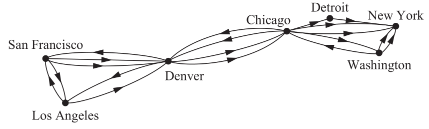
\includegraphics[scale=2]{chapter/imagens/54}
	\caption{Uma Rede de Computadores Múltiplos Links de Uma Via.}
	\label{fig54}
\end{figure}

Para alguns modelos podemos necessitar um grafo onde algums arestas não são
direccionadas, enquanto que outras são direccionadas. Um grafo com ambas arestas
direccionadas e não-direccionadas é chamado de \textbf{grafo misto}. Por
exemplo, um grafo misto pode ser utilizado para modelar uma rede de computadores
que contém ligações que operam em ambas direcções e outras ligações que operam
apenas em uma direcção.

Esta terminologia para os vários tipos de grafos é sumarizada na Tabela
\ref{tab51}. Iremos algumas vezes utilizar o termo \textbf{grafo} como um termo
deral para descrever grafos com arestas direccionadas ou não direccionadas (ou
ambos), com ou sem laços e com ou sem arestas múltiplas. Em outros casos, quando
o contexto estiver claro, iremos utilizar o termo grafo para nos referirmos
apenas aos grafos não-direccionados.

\begin{table}[H]
\centering
\begin{tabular}{|l|l|l|l|}%
\toprule
\textbf{Tipo} & \textbf{Arestas} & \textbf{Múltiplas Arestas?} &
\textbf{Laços?}
\\
\midrule
Grafo simples & Não direccionada & Não & Não \\
Multigrafo & Não direccionada & Sim & Não \\
Pseudo-grafo & Nao direccionada & Sim & Sim \\
Grafo direccionado simples & Direccionada & Não & Não \\
Multigrafo direccionado & Direccionada & Sim & Sim \\
Grafo misto & Direccionada e& Sim & Sim\\
&  \qquad não direccionada & &\\
\bottomrule%
\end{tabular}%
\caption{Terminologia dos Grafos.}
\label{tab51}
\end{table}

Por causa do recente interesse na teoria dos gradfos, e por causa da sua
aplicação à uma variedade de disciplinas, muitas terminologias da teoria dos
grados foram introduzidas. O estudante deverá determinar como tais termos estão
a ser utilizados quando os encontrar na literatura. A terminologia utilizada por
matemáticas para descrever grafos tem sido padronizada incrementalmente, mas a
terminologia usada em outras disciplinas ainda é muito variada. Embora a
terminologia usada para descrever grafos pode variar, três questões nos ajudam a
entender a estrutura de um grafo:
\begin{itemize}
  \item As arestas do grafo são não-direccionadas ou direccionadas (ou ambas)?
  \item Se o grafo é não-direccionado, existem múltiplas arestas que conectam o
  mesmo par de vértices? Se o grafo é direccionado, existem múltiplas arestas
  direccionads?
  \item Existem laços?
\end{itemize}

Responder a estas questões ajuda-nos a entender grafos independemente da
terminologia particular utilizada.


\subsection*{\underline{Modelos de Grafos}}

Grafos são utilizados numa enorme variedade de modelos. Iniciamos esta secção
por descrever como construir modelos de redes de comunicação que ligam centros
de dados. Iremos completar a secção por descrever alguns modelos diversos de
grados para algumas aplicações interessantes. Iremos retornar à algumas dessas
aplicações mais no final do capítulo. Iremos introduzir modelos adicionais de
grafos em secções subsequentes.

\begin{description}
\item[REDES SOCIAIS] Grafos são extensivamente utilizados para modelar
estruturas sociais baseadas nos diferentes tipos de relacionamentos entre
pessoas ou grupos de pessoas. Estas estruturas sociais, e os grafos que as
representam, são chamadas de \textbf{redes sociais}. Nestes modelos de grafos,
indivíduos ou organizaçãoes são representados por vértices; relacionamentos
entre indivíduos ou organizaçãoes são representadas por arestas. O estudo de
redes sociais é uma área multidisciplinar extremamente activa, e muitos
diferentes tipos de relacionamento entre pessoas foram estudados utilizando as
mesmas. Iremos apresentar algumas das mais geralmente estudadas redes sociais.

\begin{exmp}
\label{exem51}
\textbf{Grafos de Relação Pessoal e de Amizade} Podemos utilizar um grafo
simples para representar o facto de duas pessoas se conhecerem ou não, isto é, se
têm uma relação pessoal ou se são amigos (no mundo real ou no mundo
virtual através de uma rede social como o Facebook). Cada pessoa num grupo
particular de pessoas é representada por um vértice. Uma aresta
não-direccionada é usada para conectar duas pessoas quando estas pessoas
conhecem-se, ou seja têm uma relação pessoal ou se são amigos.
Não são utilizadas múltiplas arestas nem laços (se quisermos introduzir o
conceito de auto-conhecimento, acrescentaríamos laços). Um exemplo de grafo de
relação pessoal é apresentado na Figura \ref{fig55}. O grafo de relação pessoal
de todas as pessoas no mundo possui mais de seis biliões de vértices e
provavelmente mais de um trilião de arestas!
\end{exmp}

\begin{figure}[H]
	\centering
	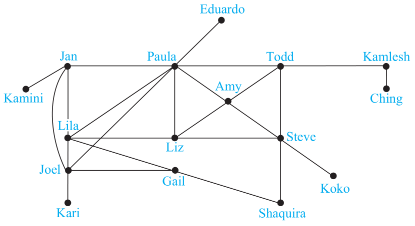
\includegraphics[scale=1.5]{chapter/imagens/55}
	\caption{Um Grafo de Relação Pessoal.}
	\label{fig55}
\end{figure}

\tikz \graph [layout=layered, radius=1cm] {
k -- j -- p -- e;
j -- l -- jl -- kr;
p -- t -- k -- c;
p -- k -- a -- s -- kk;
t -- s -- sq;
p -- lz;
a -- lz;
};

\item[REDES DE COMUNICAÇÃO]
\item[REDES DE INFORMAÇÃO]
\item[APLICAÇÕES PARA O DESENHO DE SOFTWARE]
\item[REDES DE TRANSPORTE]
\item[REDES BIOLÓGICAS]
\item[TORNEIOS]
\end{description}

\section{Terminologia dos Grafos e Tipos de Grafos Especiais}
\subsection*{\underline{Introdução}}
\subsection*{\underline{Terminologia Básica}}
\subsection*{\underline{Alguns Grafos Simples Especiais}}
\subsection*{\underline{Grafos Bipartidos}}
\subsection*{\underline{Grafos Bipartidos e Combinações}}
\subsection*{\underline{Algumas Aplicações dos Tipos de Grafos Especiais}}
\subsection*{\underline{Novos Grafos à Partir de Grados Antigos}}

\section{Representação de Grafos e Isomorfismo de Grafos}
\subsection*{\underline{Introdução}}
\subsection*{\underline{Representação de Grafos}}
\subsection*{\underline{Matrizes de Adjacência}}
\subsection*{\underline{Matrizes de Incidência}}
\subsection*{\underline{Isomorfismo de Grafos}}
\subsection*{\underline{Determinando se Dois Grafos Simples são Isomórficos}}

\section{Conectividade}
\subsection*{\underline{Introdução}}
\subsection*{\underline{Trajectória}}
\subsection*{\underline{Conectividade de Grafos Não-Direccionados}}
\subsection*{\underline{O Quão Conectado é Um Grafo}}
\subsection*{\underline{Conectividade de Grafos Direccionados}}
\subsection*{\underline{Trajectória e Isomorfismo}}
\subsection*{\underline{Contando a Trajectória entre Vértices}}

\section{Trajectória de Euler e de Hamilton}

\section{Problemas do Caminho-Mais-Curto}

\section{Grafos Planares}

\section{Coloração de Grafos}









